\section{Introduction}
\label{sec:introduction}
\IEEEPARstart{E}{dge} computing is gaining more and more attention due to the proliferation of computation-intensive and delay-sensitive mobile applications.
Edge servers are deployed in closer proximity to mobile IoT devices than the traditional cloud computing infrastructure, which enable computation offloading from mobile IoT devices (e.g., mobile phones, video surveillance cameras, etc.) via Access Points (APs) and alleviate the communication overhead. 
Since individual edge server usually has limited computation resources, distributed and collective deployment of multiple edge computing servers in the network is favored.
Therefore, a fundamental problem in edge computing is to investigate the cooperative job dispatching among multiple APs and edge servers, as illustrated in Fig.~\ref{fig:system}.
More specifically, mobile IoT devices offload their jobs through APs, each of which acts as a job dispatcher and chooses the edge server(s) to process the data. Typically, there are a large number of APs in a Metropolitan Area Network (MAN). Some APs are co-located with edge servers while others are not.

\begin{figure*}[htp!]
    \centering
    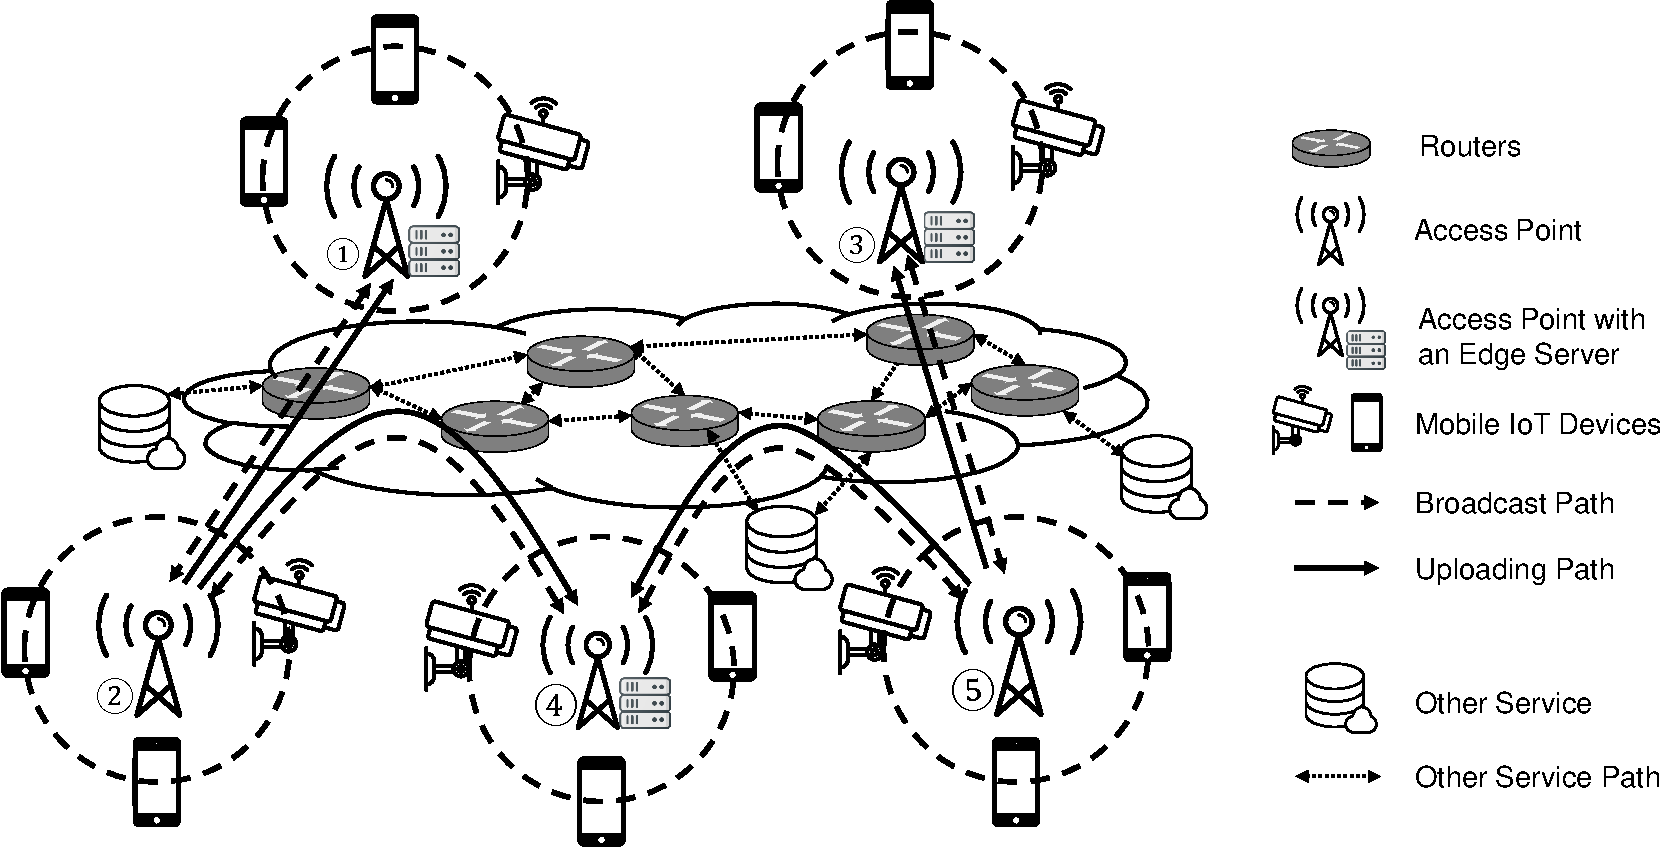
\includegraphics[width=0.60\textwidth]{hong1.pdf}
    \caption{An illustration of the system model.}
    \label{fig:system}
\end{figure*}

Most existing works assume a centralized job dispatcher which has timely and complete knowledge of the global system status and can issue the dispatching decisions to all the APs without delay \cite{tan-online,IOTJ18-FanQ,mdp-globecom,mdp-tvt,MASS18-MengZ}.
However, edge computing systems are usually deployed at Metropolitan Area Network (MAN) scale in practice, e.g., the Edge Computing Interconnect (ECI) Network \cite{MAN-ECI}, where the latency of information sharing among APs and edge servers is non-negligible. Moreover, according to the MAN performance analysis in \cite{MAN-LATENCY}, the end-to-end transmission latency is highly variable at different hours of the day and different IoT devices' locations in a MAN. This implies that there is certain randomness in the job uploading latency from APs to edge servers as well as the signaling latency (i.e., the transmission latency of the {system status} information).
There have been several works in the literature considering random transmission latency of job delivery in the edge computing network \cite{latency-EDGE19,MOBIHOC19-ZhouZ,IOTJ18-FanQ,TOC19-LiuC,JSAC19-AlameddineHA}.
However, there is relatively little work considering the random signaling latency of information sharing among distributed dispatchers \cite{tan-online,TWC18-LyuX}.
In fact, it is a challenge to consider random transmission latency in both job uploading and signaling in edge systems:
\begin{itemize}
    \item Firstly, the centralized dispatcher design is unworkable for unpredictable signaling latency, as the distribution of dispatching decisions could consume substantial extra random time. For distributed dispatchers design, however, the information exchange among distributed dispatchers also has to face up to significant signaling overhead and outdated information.
    \item Secondly, as the job arrivals at edge servers are unknown in advance because of random uploading latency, different dispatchers would have inconsistent system information even if the signaling latency is fixed.
\end{itemize}

To conclude, the random transmission latency may introduce ineliminable estimation errors on the number of jobs at APs or edge servers in the system.


In this paper, we address the above challenges by leveraging a partially observable Markov decision process (POMDP) problem formulation, and propose a novel low-complexity approximate MDP framework to solve the problem.
Specifically, we consider a practical scenario where the APs cooperatively upload different types of jobs to different edge servers with random uploading latency, and the APs receive partial system state information suffering from random signaling latency (i.e., the global system state is always partially available and outdated at the APs).
The major contributions in this paper are summarized below.
\begin{itemize}
    \item The distributed and cooperative job dispatching design with outdated and partial information is formulated as a POMDP problem.
    Different from the conventional value or policy iteration of the Bellman's equations where global or historical system states are requested in the numerical calculation, a novel low-complexity approximate MDP solution framework via \emph{alternative policy iteration} is proposed, where the dispatching policies of all APs are updated distributedly and alternatively based on a closed-form expression of the approximate local value function.
    Thus, we bypass the conventional complicated POMDP solution.
    \item We derive both the analytical performance lower bound and a tighter semi-analytical lower bound for the proposed distributed dispatching policy. In the conventional approximate MDP methods, the performance is usually evaluated numerically.
    The lower bounds not only justify the reliability of the proposed policy but also provide a method for quick performance evaluation.
    \item We extend our solution framework \algname~with an efficient online learning approach to evaluate the approximate value function when a priori knowledge of the system randomness is absent.
    \item We conduct extensive simulations based on the Google Cluster trace, and compare our approach with three heuristic benchmarks. The evaluation results show that \algname~can achieve as high as $20.67\%$ reduction in average job response time and consistently perform well under various parameter settings of signaling latency, job arrival intensity and job processing time. Moreover, the online learning algorithm has fast convergence.
\end{itemize}


The remainder of this paper is organized as follows.
In Section \ref{sec:review}, we introduce some related works about job scheduling in edge computing systems.
Section \ref{sec:model} elaborates on the system model and the signaling mechanism with random transmission latency.
In Section \ref{sec:formulation}, we formulate the global-wise optimization of dispatching decisions at all APs as a POMDP.
We propose in Section \ref{sec:algorithm} a novel low-complexity approximate MDP solution framework, called \algname.
In Section \ref{sec:rl-alg}, the solution framework is extended with reinforcement learning technique to handle the unknown statistics.
The numerical analysis of the proposed solution is presented in Section \ref{sec:evaluation}, and we conclude the work in Section \ref{sec:conclusion}.

We use the following notations throughout this paper: 
non-bold letters (e.g., $a, A$) are used to denote scalar values,
bold lowercase letters (e.g., $\mathbf{a}$) to denote column vectors,
bold uppercase letters (e.g., $\mathbf{A}$) to denote matrices,
and calligraphic letters (e.g., $\mathcal{A}$) to denote sets.
Using these notations, $\mathcal{A}\backslash\mathcal{A'}$ denotes set subtraction of $A'$ from $A$; $[\mathbf{A}]_{i,j}$ and $\mathbf{A}'$ denotes the $(i,j)$-th element and the transpose of matrix $\mathbf{A}$, respectively.

\section{Related Works}
\label{sec:review}
There have been a number of works aiming at reducing job response time by resource allocation and service migration in the edge computing system.
For example, in \cite{TON19-WangSq}, the edge servers are one-to-one bound to the base stations (BSs), and job migration could be applied according to users' mobility traces via the backhaul network connecting the BSs.
However, according to recent research \cite{INFOCOM19-WuC}, the resource re-allocation for running jobs on servers is hard to implement in practice, as it is hard for jobs to migrate among heterogeneous edge servers with different resource configurations.
Hence, it became more important to optimize the job dispatching strategy at the jobs' arrival.

There also have been some works considering centralized job dispatcher design with timely and complete knowledge of the system status.
For example, for edge computing systems with fixed uploading latency, the authors in \cite{tan-online} designed an online algorithm to minimize the average job response time in the worst case.
In the scenario that BSs and edge servers are connected via a software defined network (SDN), the authors in \cite{IOTJ18-FanQ} proposed a heuristic algorithm to dispatch the jobs to the closest edge servers according to geographical locations.
Considering random job arrivals, the authors in \cite{mdp-globecom,mdp-tvt} formulate the offloading design to a single edge server as an infinite-horizon Markov decision process (MDP).
When the jobs can be dispatched to either the edge servers or the cloud servers, the authors in \cite{MASS18-MengZ} formulated the job dispatching problem as an integer linear programming to minimize the total uploading latency.

Since centralized dispatching design might not be suitable for {edge computing systems} with distributed deployment, there are also some works addressing distributed job dispatching.
For example, in order to minimize a weighted sum of total energy consumption and uploading latency, the authors in \cite{ToN-Xuchen2016} proposed a distributed job dispatching algorithm based on game theory to achieve the Nash equilibrium. 
Considering job migration at edge servers, the authors in \cite{ToN-xujie2018} optimized the edge computing performance in a distributed manner with limited energy resources via a congestion game framework.
In a scenario that APs cooperatively dispatch jobs with multiple edge servers, the authors in \cite{mdp-jcin} proposed {an} approximate MDP method to reduce the computational complexity and minimize the average job response time.
However, in all the above works, the latency of information exchange among APs and edge servers is largely ignored.
In fact, due to the complicated network traffic, this latency might be rather significant, and the staleness {and failed transmission} of system state information at the dispatcher of edge computing systems should therefore be considered.

The staleness of information sharing among APs and edge servers may degrade the performance of the job dispatching algorithm in edge computing systems.
To the best of our knowledge, there are very limited works investigating this issue.
The authors in \cite{JSAC17-LyuX} proposed a randomized policy via a Lyapunov optimization approach to stabilize the queues in an MEC system with multiple IoT devices offloading jobs to one edge server, where \brlatency~is considered. 
In \cite{TWC18-LyuX}, the above approach was applied to the scenario where mobile devices offload jobs to each other via D2D links.
In the above two works, there is one centralized dispatcher in the system, and the objective is to stabilize the transmission queues.
Hence, the existence of \brlatency~may not pose a significant challenge to the algorithm design based on Lyapunov optimization.
In fact, the design of distributed dispatchers with \brlatency~could be more challenging.
For example, the signaling latencies at distributed dispatchers could be different significantly, and thus the synchronization of their dispatching decisions becomes infeasible.
Furthermore, taking signaling overhead and the possibility of packet drop into consideration, to make scheduling decisions based on locally observable system state information, instead of global system state information, seems more preferable.
To our best knowledge, there is no existing optimization framework appropriate for the distributed dispatcher design with both \brlatency~and partially observable system state information.

%----------------------------------------------------------------------------------------%
